% !TEX TS-program = pdflatex
% !TEX encoding = UTF-8 Unicode
\documentclass[10pt]{article}

% amsmath package, useful for mathematical formulas
\usepackage{amsmath}
% amssymb package, useful for mathematical symbols
\usepackage{amssymb}
\usepackage[english]{babel}
% graphicx package, useful for including eps and pdf graphics
% include graphics with the command \includegraphics
\usepackage{graphicx}

% cite package, to clean up citations in the main text. Do not remove.
\usepackage{cite}

\usepackage{color}

% @ACH don't know how to do this but putting this here
\usepackage{lscape}
% Use doublespacing - comment out for single spacing
%\usepackage{setspace} \doublespacing


% Text layout
\topmargin 0.0cm \oddsidemargin 0.5cm \evensidemargin 0.5cm \textwidth
16cm \textheight 21cm

% Bold the 'Figure #' in the caption and separate it with a period
% Captions will be left justified
\usepackage[labelfont=bf,labelsep=period,justification=raggedright]{caption}

% Use the PLoS provided bibtex style
\bibliographystyle{plos2009}

% Remove brackets from numbering in List of References
\makeatletter
\renewcommand{\@biblabel}[1]{\quad#1.}
\makeatother

%@CTB figure how an abbreviation for highly connected? 
%@ACH the most obvious is highly connected (HC)


% Leave date blank
\date{}

\pagestyle{myheadings}
%% ** EDIT HERE **


%% ** EDIT HERE **
%% PLEASE INCLUDE ALL MACROS BELOW

%% END MACROS SECTION

\begin{document}

% Title must be 150 characters or less
\begin{flushleft}
{\Large \textbf{Illumina Sequencing Artifacts Revealed by Connectivity
    Analysis of Metagenomic Datasets} }
% Insert Author names, affiliations and corresponding author email.
\\
Adina Chuang Howe$^{1,2}$, 
Jason Pell$^{1}$,
Rosangela Canino-Koning$^{1}$
Rachel Mackelprang$^{3}$
Susannah Tringe$^{3}$
Janet Jansson$^{3,4}$ 
James M. Tiedje$^{1,2}$
C. Titus Brown$^{1,\ast}$
\\
\bf{1} Microbiology and Molecular Genetics, Michigan State University, East Lansing, MI, USA
\\
\bf{2} Department of Plant, Soil, and Microbial Sciences, Michigan State University, East Lansing, MI, USA
\\
\bf{3} Department of Energy (DOE) Joint Genome Institute, Walnut Creek, CA, USA
\\
\bf{4} Lawrence Berkeley National Laboratory, Genomics Division, Berkeley, CA, USA
\\
$\ast$ E-mail: ctb@msu.edu
\end{flushleft}

% Please keep the abstract between 250 and 300 words
\section*{Abstract}

% @CTB revisit first sentence.  
% @ ACH Not sure what to change...switch focus to be more direct.
Sequencing errors and biases in metagenomic datasets hinder coverage-based assemblies and are often ignored during analysis.  Here, we
examine several metagenomes for the presence of sequencing
artifacts through a connectivity analysis of reads within
each metagenome's respective assembly graph.  We
identified highly connected sequences which join a large proportion of
reads within each metagenome, suggesting the presence of
non-biological biases within sequencing reads.  These sequences were
found to be biased towards specific positions within shotgun reads and
are minimally incorporated into final assemblies.  The removal of
these sequences prior to assembly results in similar assembly content
for most metagenomes, and enables the use of graph partitioning
to decrease assembly memory and time requirements.

\section*{Introduction}

With the rapid decrease in the costs of sequencing, we can now
achieve the sequencing depth necessary to study microbes from even the most complex
environments \cite{Hess:2011p686,Qin:2010p189}.  Deep
metagenomic sequencing efforts in permafrost soil, human gut, cow
rumen, and surface water have provided insights into the genetic and
biochemical diversity of environmental microbial populations
\cite{Hess:2011p686,Iverson:2012p1281,Qin:2010p189} and how
they are involved in responding to environmental changes
\cite{Mackelprang:2011p1087}. These metagenomic studies have all
leveraged \emph{de novo} metagenomic assembly of short reads for
functional and phylogenetic analyses
\emph{De novo} assembly is
an advantageous approach to sequence analysis as it reduces the
dataset size by collapsing the more numerous short reads into fewer contigs and
enabling better annotation-based approaches by providing longer sequences.
\cite{Miller:2010p226,Pop:2009p798}
Furthermore, it does not rely on the a priori availability of
reference genomes to enable identification of novel genetic features
and construction of draft genomes \cite{Hess:2011p686,Iverson:2012p1281}.
% @CTB what does ``enabling identification ... of draft genomes'' mean?
% @ ACH added "construction of"

Although \emph{de novo} metagenomic assembly is a promising approach
for metagenomic sequence analysis, it is complicated by the variable
coverage of sequencing reads from mixed populations in the environment
and their associated sequencing errors and biases
\cite{Mende:2012p1262,Pignatelli:2011p742}. Several
metagenome-specific assemblers have been developed to deal with
variable coverage communities, including Meta-IDBA
\cite{Peng:2011p898}, MetaVelvet, and SOAPdenovo (cite).  These assemblers
rely on analysis of local sequencing coverage to help build assemblies
and thus are sensitive to the effects of sequencing errors and biases
on coverage estimations of the underlying dataset. The effects of
sequencing errors on \emph{de novo} assembly has been demonstrated in
simulated metagenomes
\cite{Mavromatis:2006p894,Mende:2012p1262,Pignatelli:2011p742} or
isolate genomes \cite{Morgan:2010p740}, but these datasets do not
incorporate models that are representative of real metagenomic data.
Specifically, these models exclude the presence of known
non-biological sequencing biases
\cite{GomezAlvarez:2009p1334,Keegan:2012p1336,Niu:2010p1333} which
hinder assembly approaches.
% @CTB also remember to discuss polymorphism
% @CTB for isolated genomes, add Chitsaz citation.

In this study, we examine metagenomic datasets for the presence of
artificial sequencing biases that affect assembly graph structure,
extending previous work to large and complex datasets produced from
the Illumina platform. We characterize sequence connectivity in an
assembly graph, identifying potential sequencing biases in regions
where numerous reads are connected together.  Within metagenomic
datasets, we find that there exist highly connected sequences which
partially originate from sequencing artifacts.  Moreover,
these sequences limit approaches to divide or partition large datasets
for further analysis, and may introduce artifacts into assemblies.  Here, we
identify and characterize these highly connected
sequences, and examine the effects of removing these sequences on
downstream assemblies.

\section*{Results}

\subsection*{Connectivity analysis of metagenome datasets}

\subsubsection*{Presence of a single, highly connected lump in all datasets}
We selected datasets from three medium to high diversity
metagenomes from the human gut \cite{Qin:2010p189}, cow rumen
\cite{Hess:2011p686}, and agricultural soil (SRX099904 and SRX099905)
(Table 1).  To
evaluate the effects of sequencing coverage, we included two subsets
of the 520 million read soil metagenome containing 50 and 100 million
reads.  We also included a previously published error-free simulated
metagenome based on a mixture of 112 reference genomes
\cite{Pignatelli:2011p742}.

% @CTB refactor paragraph: using a DBG, cite Pell, etc.
Initially, we evaluated the amount of connectivity between all
sequences in each metagenome using an approach similar to the initial
step of short read assemblers to identify overlaps of short sequences
of length 'k', or k-mers
\cite{Peng:2011p898,Simpson:2009p233,Zerbino:2008p665}.  For complex
metagenomes, large amounts of memory are required to store reads and
their associated sequencing errors in assembly graphs
\cite{Hess:2011p686,Mackelprang:2011p1087,Qin:2010p189}.  To overcome
this limitation, we constructed a probabilistic representation of the
assembly graph using a bloom filter de Bruijn graph representation
within fixed memory as previously described (Pell et al, how to cite
this?).
% @CTB cite

Using this assembly graph representation, we separated reads
contributing to disconnected portions of the metagenome assembly graph.
For each metagenome, regardless of origin, we found a
single dominant, highly connected set of sequencing reads which we
henceforth refer to as the ``lump'' of the dataset (Table 1, column
3).  This lump contained the largest subset of connected sequencing
reads and varied in size among the datasets, ranging from 5\% of total
reads in the simulated metagenome to 75\% of total reads in the human
gut metagenome.  For the soil datasets, as sequencing coverage (e.g.,
the fraction of reads mapped to an assembly) increased from 1.4 to 4.7
to 5.6\%, the lump size increased more dramatically from 7 to 15 to
35\% of all reads, indicating increasingly larger connectivity between
sequences with more sequencing.

\subsubsection*{Characterizing the connectivity in the dominant lump}

% @CTB check scripts to see if this is an accurate characterization.
% @CTB put scripts in scripts/!!
We characterized the connectivity of sequences
within each lump by estimating the average local graph density from
each k-mer (k=32 unless otherwise stated) in the assembly graph (see
Methods).  Here, local graph density is a measurement of total
connected reads within a fixed radius.  Sequences
in the identified metagenomic lumps were characterized by very high
local graph densities: between 22 to 50\% of the total nodes in
metagenomic lump assembly graphs had average graph densities greater
than 20 (Table 1).  This means that these nodes were in very nonlinear portions of the assembly graph and had high connectivity.  In comparison, 17\% of the total nodes in the
simulated lump had an average local graph density greater than 20, and
fewer than 2\% of the nodes in the entire simulated data set had an
average graph density higher than 20.

We next assessed the extent to which graph density varied by position
along the sequencing reads.  The degree of position-specific variation of
graph densities was estimated by calculating the average local graph
density within ten steps of every k-mer by position in each read.  In
all environmental metagenomic reads, we observed variation in graph
density at the 3'-end region of reads (Figure 1).  In soil
metagenomes, we observed the most dramatic variation with local graph
density increasing in sequences located at the 3'-end of the reads.
Notably, this trend was not present in the simulated dataset.

Next, we performed an exhaustive traversal of the assembly graph and
identified the specific sequences within dense regions of the assembly
graph which consistently contributed to high connectivity.  We
observed that this subset of sequences was also found to exhibit
position-specific variation within sequencing reads, with the
exception of these sequences in the simulated dataset (Figure 1, solid
lines).  Similar to local density trends, position-specific trends in
the location of these sequences also varied between metagenomes.  As
sequencing coverage increased among metagenomes, the amount of 3'-end
variation appeared to decrease (e.g., the soils) or inverse (e.g.,
rumen and human gut).

\subsection*{Effects of removing highly connected sequences on assembly}

\subsubsection*{Removal of highly connected sequences enables graph partitioning of metagenome}

Since these highly connected sequences exhibited position-specific
variation indicative of sequences of non-biological origin, we removed
them and assessed the effect of their removal on assembly
(see Methods).  We
found that by removing these k-mers, we could effectively break apart
metagenomic lumps, and the resulting largest partition of connected
reads in each metagenome was reduced to less than 7\% of the total
reads in the lump.  As a consequence of partitioning the metagenomic
lump, we were able to greatly reduce assembly requirements.
% @CTB refactor below
Compared
to unfiltered datasets which required greater than 100 GB and 100
hours in the case of the largest soil metagenome (Table 2), all
partitioned datasets could be assembled in less than 2 GB of memory
and less than 1 hour using multiple nodes.

\subsubsection*{Removal of highly connected sequences resulted in minimal losses of reference genes}

% @CTB probably need to indicate that since lump is separated from rest
% we can assemble it separately w/o fear.
We explored the extent
to which the identified highly connected
sequences impacted assembly by first evaluating the effects of the
removing these sequences from the simulated lump.  The assembly of the reads in the original,
unfiltered simulated lump and that of the reads remaining after
removing highly connected sequences (the filtered assembly) were
compared for three assemblers: Velvet, Meta-IDBA, and SOAPdenovo.
Based on the total assembly length of contigs greater than 300 bp,
filtered assemblies of the simulated metagenome resulted in a loss of
between 4 - 16\% of total assembly length (Table 2).  In general, the
filtered assemblies contained fewer total contigs than unfiltered
assemblies, and the maximum contig size increased in the Velvet
assembly but decreased in the Meta-IDBA and SOAPdenovo assemblies.
Direct comparisons of the unfiltered and filtered assemblies found
that the filtered assemblies comprised on average 88\% of the
unfiltered assemblies, and the unfiltered assemblies contained nearly
all, 96\%, of the filtered assembled sequences.  Despite the removal
of over 3\% of the total unique 32-mers in the simulated metagenome,
the resulting filtered assemblies resulted in only a loss of 0.1 -
0.6\% of annotated original reference genes (Tables 1 and 2).
% @@CTB was normalized blast used here?
%@ACH Yes, the coverage-blast script with slight modification to only take hits with evalue < 1e-5.

We next evaluated the effects of using similar approaches on
real datasets.  Similar to the simulated assemblies, the
removal of highly connected sequences for all metagenomes and
assemblers resulted in a decrease of total number of contigs and assembly
length (Table 2).  In general, filtered assemblies were largely
contained within unfiltered assemblies and comprised 51-88\% of the
unfiltered assembly.  The observed changes in metagenomic assemblies
were difficult to evaluate as no reference genomes exist, 
and a decrease in assembly length may actually be beneficial if it
eliminates contigs that incorporate sequencing artifacts.
To aid in this evaluation, we used the previously published set of
rumen draft genomes from \emph{de novo} assembly efforts of high
abundance sequences in the rumen metagenome \cite{Hess:2011p686}.
Overall, we found that removal of highly connected sequences from the
rumen dataset resulted in 1-3\% loss of sequences which matched to
draft reference genomes (Table 2).
% @CTB note that the rumen genomes may not be correct
% @CTB also be sure to discuss why assemblies might differ (length cutoff stuff)

\subsubsection*{Unfiltered assemblies contained only a small fraction of highly connected sequences}
To further study the effects of highly connected sequences, we
examined their incorporation into unfiltered assemblies.  Except in
the human gut sample, fewer than 2\% of highly connected sequences
were incorporated by any assembler (Table 1 and 3).  Each assembled
contig was divided into equal length bins (the size of bins was
dependent on the total length of the contig) and examined for the
presence of the previously identified highly connected sequences.  We
found that contigs, especially in assemblies from Velvet and
Meta-IDBA, incorporated a larger fraction of these sequences at their
ends relative to other positions (Figure 3).  The SOAPdenovo
assembler incorporated fewer of the highly connected sequences into
its assembled contigs; none of these sequences in the simulated
dataset were assembled, and only 41 in the small soil dataset.  For
the human gut metagenome assemblies, millions of the highly connected
sequences were incorporated into assembled contigs, comprising nearly
4\% of all assembled sequences on Velvet contig ends (Figure 4,
suggestion to move to supp figures -- YES CTB).
% @CTB do we want to talk about end bins or percentile bins?  Probably fine
% to leave as is.

\subsubsection*{Identifying origins of highly connected sequences in known reference databases}

For the simulated metagenome, we could identify the source of highly
connected k-mers using available reference genomes. Reference genes
with multiple perfect alignments to highly connected k-mers present in
the dataset a minimum of 50 times were identified (Table 4).  Many of
these sequences were from well-conserved housekeeping genes involved
in protein synthesis, cell transport, and signaling.  To determine
possible biological sources of highly connected sequences within real
metagenomes, we compared the sequences shared between the soil, rumen,
and human gut metagenomes (a total of 241 million 32-mers).  For these 7,586 shared sequences, we identified the closest reference
protein from the NCBI-nr database requiring complete sequence
identity.  Only 1,018 sequences (13\%) matched existing reference
proteins, and many of the annotated sequences matched to
genes conserved across multiple genomes.  The top five
proteins conserved in greater than 3 genomes are shown in Table 4, and
largely encode for genes involved in protein biosynthesis, DNA
metabolism, and biochemical cofactors (Table 5).
% @CTB yes, out of of how many k-mers?
% @ ACH the largest soil genome had the most unique kmers and had 737000 kmers
% @CTB what is our conclusion here, anyway, about the origin?
% @ ACH - Origins are for the most part not systematic (not shared) and not in NR database, indicative of artifactual origin.
% @CTB what does ``top five'' mean here -- abundance?
% @ ACH Top Five, proteins with the most BLAST hits 

One potential cause of artificial high connectivity within metagenomes
is the presence of high abundance subsequences.  Thus, we identified the
subset of highly connected k-mers which were also present with an
abundance of greater than 50 within each metagenome and their location
in sequencing reads (Figure 2, dotted lines).  These high abundance
k-mers comprised a very small proportion of the identified highly
connected sequences, less than 1\% in the soils, 1.5\% in the rumen,
and 6.4\% in the human gut metagenomes, but the position-specific
variation of these sequences was very similar to the variation in the
larger set of highly connected k-mers.
% @CTB was diginorm used for abundance > 50?
% @ACH No, diginorm was not used for anything here.  The stop tags were identified by graph traversal and then HA abundance were identified among those.

To identify consistent patterns within sequences causing
position-specific variation, we examined the abundance distribution of
5-mers contained within the high abundance subset of each dataset's
highly connected 32-mers.  There were significantly fewer 5-mers in
the simulated sequences compared to those in metagenomes: 336 5-mers
in the simulated and 425,572 to 221,085,228 in the small soil and
human gut datasets, respectively.  We examined the distribution of the
abundance of these 5-mers, evaluating any significant presence of
specific 5-mers.  In the simulated dataset, the top ten most abundant
unique k-mer made up 75\% of the total 5-mers; in contrast, in the
metagenomes, the top ten most abundant 5-mers comprised less than 10\%
of the total 5-mers.  When the 5-mers in each metagenome dataset were
ranked from highest to lowest abundance, all sequences represented an
even distribution of total cumulative k-mers, and the opposite trend
is observed in the simulated dataset where the majority of 5-mers are
among the most abundant.
% @CTB what does this mean? do we say anywhere?
% @ACH This was kinda an extra analysis to look for patterns in the k-mers, something that was not restricted to a database blast as done above.  It means that there are no patterns that we can find that are systematic.
% @CTB somewhere we should put in extra discussion about why k-mers are
% so important :)

\section*{Discussion}

\subsection*{Sequencing artifacts are present in highly connected sequences}

Through assessing the connectivity of reads in several metagenomes, we
identified a disproportionately large subset of reads
connected together within an assembly graph, which we refer to as
the ``lump''.
The total number of reads in
metagenomic lumps (7-75\% of reads) was significantly larger than that
of simulated dataset (5\% of reads) (Table 1).  As the simulated
dataset contains no errors, this observed connectivity represents
conserved sequences within a single genome or between multiple genomes
(specific genes identified in Table 4).  The larger size of the highly
connected lump within the soil, rumen, and human gut metagenomes
suggests that anomalous, non-biological connectivity may be present
within these lumps.  Interestingly, in the soil metagenomes, we
observed that the amount of connectivity nearly doubled with less than
a 5\% increase of sequencing coverage.  When sequencing coverage
increased slightly from 4.7 to 5.6\% in the medium and large soil
metagenomes, the number of reads connected in the lump grew
significantly from 15 million to 182 million.  Given the very high
diversity and very low coverage of these soil samples, the magnitude of the
observed increases in connectivity seemed unlikely to originate from biological
sources, further suggesting the presence of sequencing biases within
these datasets.
% @CTB what does ``a 5% increase of sequencing coverage'' mean? in reads?
% or reads mapped to assembly?  
% @ACH - Yeah, we should be clear about the nomenclature here, I don't know what it should be but it is % of reads mapped to the assembly.

If sequencing biases were present within these metagenomes, we would
expect that the metagenomic lumps would consist not only of
artificial sequences but also sequences from reads which would be
``preferentially attached'' \cite{Barabasi:1999p1083}.  Consider that
there is an original set of highly connecting ``X'' sequences in a
lump.  These sequences would recruit a number of connected ``Y'' reads
into the lump.  These recruited ``Y'' reads would then recruit more
``Z'' reads into the lump which would not necessarily connect to the
original ``X'' reads.  In error-free datasets, we would observe this
preferential attachment phenomenon as a linear increase of lump size
with increasing sequencing coverage.  In the case of the presence of
highly connected sequencing biases, however, we'd observe that
preferential attachment would cause dramatic increases in the number
of recruited ``Y'' and ``Z'' reads, as is observed in the soil
datasets.
% @CTB rewrite

The sequencing of metagenomes is a random
process and consequently any position-specific variation within sequencing
reads is unexpected and probably originates from bias in sample preparation
or the sequencing process (cite).  For the metagenomes
studied here, we used two approaches to examine characteristics of
connectivity correlated to specific positions within sequencing reads.
First, we measured the connectivity of sequences at specific positions
within reads by calculating local graph density.  Next, we identified
the specific k-mers which were consistently present in highly dense
regions of the assembly graph and evaluated their location within
sequencing reads.  When these approaches were applied to the simulated
dataset, we observed no position-specific trends when assessing either
local graph density (Figure 1) or highly connected k-mers (Figure 2,
solid lines) as is consistent with the lack of sequencing errors and
variation in this dataset.  In all real metagenomes, however, we
identified position-specific trends in measurements of both local
graph density and the location of highly connected sequences, clearly
indicating the presence of artificial sequences.  Although present in
all metagenomes, the direction of the variation varied between soil, rumen,
and human gut datasets, especially for the position-specific presence
of identified highly connected sequences.  It is likely that there is
a larger presence of indirectly preferentially attached reads which
are connected to high coverage sequences of biological origins in
higher coverage datasets, such as the rumen and human gut.  This
preferential attachment of such reads would result in increasing the
number of total reads and consequently the decrease the total fraction
of highly connected k-mers (Figure 2, y-axis).  This trend is observed
in the decreasing fractions of highly connected sequences at the 3'
end of reads as sequencing coverage increased in the small, medium, to
large soil metagenomes and in the soil, rumen, to human gut
metagenomes (Figure 2).
% @CTB is this last bit bullshit or not?  Speculate on ligation efficiency
% etc. :)

\subsection*{Assessing the validity of removing highly connected sequences from metagenomes}

% @CTB refactor roundabout section title
\subsubsection*{Highly connected sequences are difficult to assemble}

% @CTB refactor
As is apparent from conserved biological sources of high connectivity
within the simulated metagenome, not all the observed connectivity
within real metagenomes is artificial, and our approaches are limited
in that they cannot differentiate between sequencing artifacts and
sources of real biological connectivity.  Regardless of the origin of
highly connected sequences, we suspected that these sequences would
challenge assemblers which rely on traversing the complex ``lump'' in
the assembly graph.  Indeed, very few highly connected sequences with
abundances greater than 50 were incorporated into contigs (Table
3). Moreover, those which were assembled were often disproportionately placed
at the ends of contigs (Figure 3), suggesting that they confused the
assembly process.  Although this trend was
observed for all assemblers, it was more prevalent in the Velvet and
Meta-IDBA assemblers, highlighting differences in assembler
heuristics.

\subsubsection*{Removing highly connected sequences enabled more efficient assembly of partitioned reads}

Since these highly connected sequences contained artifacts and 
were challenging for assemblers,
we assessed the
effects of removing them for the assembly of metagenomic lumps.  We
found that removal of these highly connected sequences had two key
advantages: first, it removed artificial sequences which should not be
assembled, and second, it resulted in the dissolution of the high
connectivity within the metagenomic lump and consequently allowed for
the partitioning of all metagenomes.  We compared the combined
assembly of the partitioned sets of filtered reads to the original
lump dataset with several assemblers.  For the partitioned reads, we
were able to assemble subsets of reads in parallel, resulting in
significantly reduced time and memory requirements for assembly (Table
2).  In the case of the largest soil metagenome (containing over 500
million reads), we could not complete the Meta-IDBA assembly of the
unfiltered reads in less than 100 GB of memory, but after removing
highly connected sequences and partitioning, the assembly could be
completed in less than 2 GB of memory.  Using partitioned sets of
reads for all metagenomes, we were also able to efficiently complete
multiple k-mer length assemblies (demonstrated with Velvet) and
subsequently merge resulting assembled contigs.  For unfiltered
datasets, this was previously either impossible (due to memory
requirements) or impractical (due to time).

We used consistent parameters (i.e. k-length, estimations of coverage,
etc.) to compare assemblies, but it is often beneficial to optimize
these values to characteristics of the underlying dataset.
Partitioning metagenomic reads based on connectivity effectively
divides the cumulative environmental dataset into subsets representing
fragments from different genomes.  Thus, partitioning enables
optimization for a single population subset (rather than a community
metagenome) for assembly and many other analyses (i.e. binning,
annotation, SNP identification).  Additionally, because the partitions
are manageable in size, it is practical to complete multiple
assemblies to evaluate different assemblers and/or assembly
parameters.  As metagenome datasets grow increasingly larger, this
ability to efficiently analyze datasets and/or evaluate multiple
assemblies will be increasingly important.
% @CTB do we show that we are dividing things up into different genomes?
% @ACH - No not here, but we do in the assembly #2 paper.  I dont know if we should put too much in here re this.

\subsubsection*{Removal of highly connected sequences prior to assembly did not result in significant loss of reference genes}
The advantages of removing highly connected sequences must be balanced
against consequences to resulting assemblies.  We compared several
metagenome assemblies before and after the removal of these sequences.
Comparing the simulated dataset's assemblies, the removal of highly
connected sequences resulted in very little loss of annotated
reference genes (less than 1\%) and a similar assembly compared to the
unfiltered data (~85\% similarity), supporting the removal of these
highly connected sequences especially for gains in assembly
efficiency.  For the rumen metagenome, we performed a partial
evaluation of the assemblies using available draft reference genomes.
Similar to the simulated assemblies, we observed only a small loss
(less than 3\%) of rumen reference genomes assembled (Table 2).  In
general, for all metagenomes, we observed ~25\% loss in assembly after
removing highly connected sequences, much more than observed in
assemblies of reference genes and genomes in the simulated and rumen
datasets.  Some of this loss is likely beneficial, resulting from
removal of sequencing artifacts; it is also possible that our approach
removes sequences which can accurately be assembled, but we cannot
evaluate this in the absence of reference genomes.
However, without the
removal of these sequences, many of the assemblies of the larger
metagenomes would not be practical.

\subsection*{Highly connected sequences do not match known reference sequences}

We attempted to identify biological characteristics of highly
connected sequences.  Among these sequences in the simulated dataset
and those shared by all metagenomes, we identified only a small
fraction (13\% in simulated and less than 7\% in metagenomes) which
matched reference genes associated with core biological functions
(Tables 4 and 5).  This suggests that the remaining sequences are
either not present in known reference genes (i.e., conserved
non-coding regions) or originate from non-biological sources.  This
supports the removal of these sequences for typical assembly and
annotation pipelines, where assembly is often followed by the
identification of protein coding regions.

Speculating that many of the highly connected sequences originated
from high abundance reads, we examined the most abundant subsequences.  We found
that these subsequences (present greater than 50x) displayed similar
trends for position-specific variation compared to their respective sets
of highly connected subsequences (Figure 2), indicating that they
contribute significantly to position-specific variation.  We attempted to
identify signatures in the the abundant, highly connected sequences of
the simulated and metagenomic datasets.  In the simulated dataset, we
found that the total number of unique 5-mers was significantly lower
than that in metagenomes and that the most abundant of these 5-mers
comprised the large majority of the total.  This result is consistent
with the identification of conserved biological motifs in the
simulated dataset which would result in a small number of highly
abundant sequences.  In contrast, within metagenomic data, we found
that the 5-mersse are evenly distributed and random in metagenomes
(Figure 5), making them difficult to identify and evaluate.
Currently, we are evaluating a promising approach to improve the
identification and removal of probable sequencing artifacts based on
targeting high abundance sequencing.
% @CTB this is the diginorm abundance removal, right? should we keep this in? 
%@ACH okay with me to chuck it.

\section*{Conclusion}

As datasets from NGS technologies continue to increase in size,
current analysis approaches are no longer adequate.  In this study, we
characterize the connectivity of sequences in several metagenomes to
better understand how we can improve approaches towards {\em de novo}
metagenomic assembly.  We demonstrate the existence of extremely
highly connected sequences within several metagenomes and show that
they are comprised of sequencing artifacts.  These sequences add
erroneous diversity and high coverage to datasets and significantly
increase memory requirements for assembly.  We show that assemblers
are challenged by these sequences and that their removal results in
comparable assemblies and enables partitioning of complex metagenome
assembly graphs into disconnected subsets, allowing low-memory
execution of previously impractical to complete assemblies.  Our
analysis provides an understanding of the nature of highly connected
sequences in metagenomes and suggests that their removal is an
important first step for scalable \emph{de novo} assembly.  This study
highlights the importance of re-evaluating the nature of new
sequencing data for both accurate and efficient downstream analysis
approaches.
% @CTB we don't really emphasize scalability anywhere else, do we?


\section*{Methods}

\subsection*{Metagenomic datasets}
All datasets, with the exception of the agricultural soil metagenome,
originate from previously published datasets. Rumen-associated
sequences (Illumina) were randomly selected from the rumen metagenome
available at ftp://ftp.jgi-psf.org/pub/rnd2/Cow\_Rumen
\cite{Hess:2011p686}. Human-gut associated sequences (Illumina) of
samples MH0001 through MH0010 were obtained from
ftp://public.genomics.org.cn/BGI/gutmeta/ Raw\_Reads
\cite{Qin:2010p189}.  The simulated high complexity, high coverage
dataset was previously published \cite{Pignatelli:2011p742}.  All
reads used in this study, with the exception of those in simulated
metagenome, were quality-trimmed for Illumina's read segment quality
control indicator, where a quality score of 2 indicates that all
subsequent regions of the sequence should not be used. After
quality-trimming, only reads with lengths greater than 30 bp were
retained. All quality trimmed datasets, including the previously
unpublished agricultural soil metagenome, are available on a public
Amazon EC2 snapshot (snap-ab88dfdb).  The sequencing coverage of each
metagenome was estimated as the fraction of reads which could be
aligned to assembled contigs with lengths greater than 500 bp.  For
the coverage estimates, an assembly of each metagenome was performed
using Velvet (v1.1.05) with the following parameters: K=33, exp
cov=auto, cov cutoff=0, no scaffolding.  Reads were aligned to
assembled contigs with Bowtie (v0.12.7), allowing for a maximum of two
mismatches.

\subsection*{Lightweight, compressible de Bruijn graph representation}
We used a lightweight probabilistic de Bruijn graph representation to
explore k-mer connectivity of the assembly graph (cite PNAS paper,
software available at https://github.com/ctb/khmer). The de Bruijn
graph stores k-mer nodes in Bloom filters and keeps edges between
nodes implicitly.  For metagenomes in this study, we used 4 x 48e9 bit
bloom filters to store connectivity of the assembly graphs.  We
partitioned disconnected subsets of the assembly graph, and the set of
the largest number of reads which were connected in the assembly graph
is referred to above as a single, highly connected lump.  Data and
examples of scripts used for this analysis are available on the Amazon
EC2 public snapshot: data-in-paper/lumps and
method-examples/0.partitioning-into-lump.
% @CTb we need to tag & freeze a particular khmer version.  What version?
%@ACH - The most recent one should be fine to freeze. commit 22674158d57dabe7d3f7ef480c713ade1daf6f84
\subsection*{Local graph density and identifying highly connected k-mers}
We implemented a systematic traversal algorithm to identify highly
connected components of the assembly graph.  Waypoints were labeled to
cover the graph such that they are a minimum distance of L
apart. Originating from a waypoint, all k-mers (throughout the study
k=32 unless otherwise stated) were systematically and exhaustively
traversed within a region that is the distance N.  The local graph
density was calculated as the number of X k-mers reachable within a
distance of N nodes (k-mers) divided by the distance N.  In this
study, N was equal to 10 nodes within the assembly graph.  For the
largest metagenomes, the human gut and large soil datasets, local
graph density was calculated on a representative subset of reads due
to computational limitations.  To identify specific highly connected
sequences within the lump assembly graphs, graph traversal to a
distance of 40 nodes was attempted from marked waypoints.  If more
than 200 k-mers were found within this traversal were identified, all
k-mers within this traversal were identified as candidates for highly
connected sequences.  If the same k-mers were consistently identified
in other graph traversals, up to five times, the k-mer was flagged as
a highly connected sequence.  Aligning theses k-mers to original
sequencing reads, we identified the position-specific location of
these k-mers.  Data and examples of scripts used for this analysis are
available on the Amazon EC2 public snapshot:
data-in-paper/density-bias, data-in-paper/hc-kmer-bias,
method-examples/1.density-analysis,
method-examples/2.identifying-hc-kmers, and
method-examples/3.hc-kmer-analysis.

To identify the sources of highly connected k-mers identified in the
simulated metagenome, these sequences were aligned against the
reference genes originating from the 112 source genomes using Bowtie
(v0.12.7) requiring exact matches.  highly connected k-mers shared
between all the metagenomes were also aligned against the NCBI
non-redundant genome database (ftp://ftp.ncbi.nih.gov/blast/db, March,
1, 2011) using blastn \cite{Altschul:1990p1335} and requiring an exact
match over the entire k-mer.  Genes which matched highly connected
sequences and were conserved among genome(s) were identified (Tables 4
and 5).

We also identified the subset of highly connected k-mers which were
present at greater than 50 times within lumps. Data used for this
analysis are available on the Amazon EC2 public snapshot:
data-in-paper/lumps/HC-kmers/HA-HC-kmers and
method-examples/4.abundant-hc-kmers. These high abundance, highly
connected sequences were aligned to sequencing reads to demonstrate
position specific variation as described above.  We evaluated the
existence of short k-mer (k=5) motifs within high abundance, highly
connected k-mers which did not have an exact match to the NCBI
non-redundant database.  Each identified 32-mer was broken up into
shorter 5-mers, and the frequency of each unique 5-mer was calculated.
Next, each unique 5-mer was ranked based on its abundance, from high
to low, and the cumulative percentage of total 5-mers is shown in the
resulting rank-abundance plot (Figure 5).
  
\subsection*{\emph{De novo} metagenomic assembly}

The lump within each dataset was assembled and referred to as the
``unfiltered assembly''.  Additionally, highly connected sequences
identified as described above were were trimmed from sequencing reads
and the remaining reads partitioned and assembled, resulting in the
``filtered assembly''.  \emph{De novo} metagenomic assembly of reads
was completed with Velvet (v1.1.02) with the following parameters:
velveth -short -shortPaired (if applicable to the dataset) and velvetg
-exp\_cov auto -cov\_cutoff 0 -scaffolding no \cite{Zerbino:2008p665}.
For the small and medium soil, rumen, and simulated datasets, Velvet
assemblies were performed at K=25-49, resulting contigs were
dereplicated to remove contigs with 99\% similarity using CD-HIT (v
4.5.6, \cite{Li:2001p1337}), and final contigs were merged with
Minimus (Amos v3.1.0, \cite{Sommer:2007p1253}).  For the largest soil
and human gut metagenomes, assemblies were performed at only K=33 due
to the size of the datasets and memory limitations.  Additional
assemblies were performed with meta-IDBA (v0.18) \cite{Peng:2011p898}
: --mink 25 --maxk 50 --minCount 0 and with SOAPdenovo: -K 31 -p 8
max\_rd\_len=200 asm\_flags=1 reverse\_seq=0.  After removal of highly
connected k-mers in metagenomic lumps, each filtered lump was
partitioned into separate disconnected subgraphs.  Multiple subgraphs
were grouped together such that assembly could be performed in
parallel on groups of sequences.  Identical assembly parameters and
methods as described above were used for these assemblies.  Unfiltered
and filtered assemblies were compared using the total number of
contigs, total assembly length, and maximum contig size.  Additional,
the coverage of each assembly was calculated through estimating the
average base pair coverage of the BLAST alignment of each assembly to
one another (E-value greater than 10$^{-5}$) or, in the case of the
simulated and rumen assemblies, to reference genomes.  The simulated
and rumen reference genomes were previously published in
\cite{Hess:2011p686} and \cite{Pignatelli:2011p742}, respectively.
Resulting assemblies are available on the Amazon EC2 public snapshot:
/data-in-paper/assembly*.

We examined incorporation and the location of the identified high
abundant, highly connecting k-mers within assembled contigs.
Incorporation of these sequences was evaluated by dividing assembled
contigs into words of 32 bp length and identifying exact matches
between sequences and contig fragments.  The location of these k-mers
within assembled unfiltered contigs was examined by dividing each
contig into 100 equally-sized regions.  The fraction of highly
connecting k-mers which aligned exactly to each region was calculated
for each metagenome. Data and examples of scripts used for this
analysis are available on the Amazon EC2 public snapshot:
method-examples/5.hc-kmer-contigs/.



\bibliography{artifacts-bib}


\pagebreak

\begin{landscape}
\begin{table}[ht]
\centering
\caption{The original size and proportion of highly connective 32-mers in the largest subset of partitioned reads (``lump'') in several medium to high complexity metagenomes.  Read coverage was estimated with the number of aligned sequencing reads to Velvet-assembled contigs (K=33).  The dominant lump, or largest disconnected component of each metagenome assembly graph, was found to contain highly connecting k-mers responsible for high local graph density.}
\begin{tabular}{lp{2cm}cp{2cm}cp{2cm}cp{2cm}cp{2cm}cp{2cm}cp{2cm}cp{2cm}cp{2cm}|}
\hline
& Reads	& Mapped to assebmly	& Lump reads	& Highly connective & Total & Highly connective  & Density \textgreater 20  \\
& (millions) & (percent) & (millions) & (32-mers) & (32-mers) & (percent) & (percent) \\

\hline
Small Soil 	& 50.0 	& 1.4 	& 3 .0 (7\%)	& 6,429,673 	& 84,906,521 	& 8\% 	& 50\% \\
Medium Soil 	& 100.0 	& 4.7 	& 15.0 (15\%)	& 33,266,397 	& 326,454,473 & 10\% 	& 37\% \\ 
Large Soil	 	& 520.3 	& 5.6 	& 182.2 (35\%)	& 230,353,299 & 2,198,140,432 & 10\% 	& 40\% \\
Rumen 		& 50.0 	& 32.0 	& 10.3 (21\%)	& 25,400,121 	& 201,532,081 	& 13\% 	& 22\% \\
Human Gut 	& 350.0	& 3.5 	& 263 (75\%) 	& 136,594,783	 & 860,627,857 & 16\% 	& 28\% \\
Simulated		& 9.2		 & 14.8 	& 0.5 (5\%) 	& 364,816 	& 11,592,284 	& 3\% 	& 17\% \\
\hline
\end{tabular}
\end{table}
\end{landscape}

\begin{landscape}
\begin{table}[ht]
\caption{Comparison of unfiltered (UF) and filtered (F) assemblies of various metagenome lumps using Velvet, SOAPdenovo, and Meta-IDBA assemblers.  Assemblies were aligned to each other, and coverage was estimated (columns 1-2).  Simulated and rumen assemblies were aligned to available reference genes (RG)/genomes (columns 3-4).}

\begin{tabular}{*{5}{p{3cm}}}
Velvet Assembler  \\ 
\hline
& Cov. of UF by F & Cov. of F by UF  & Cov. of RG  by UF  & Cov. of RF by F \\
\hline
Small Soil		&74.5\%		&98.6\%		&-		&-\\
Medium Soil	&75.4\%		&98.1\%		&-		&-\\
Large Soil		&50.8\%		&86.3\%		&-		&-\\
Rumen		&75.1\%		&98.3\%		&17.2\%	&14.6\%\\
Human Gut 	&79.5\%		&88.5\%		&-		&-\\
Simulated		&84.6\%		&98.3\%		&4.5\%	&3.9\%\\
\end{tabular}

\begin{tabular}{*{5}{p{3cm}}}
Meta-IDBA Assembler  \\ 
\hline
& Cov. of UF by F & Cov. of F by UF  & Cov. of RG  by UF  & Cov. of RF by F \\
\hline
Small Soil		&75.6\%		&93.9\%		&-		&-\\
Medium Soil	&67.5\%		&94.5\%		&-		&-\\
Large Soil		&N/A			&N/A			&-		&-\\
Rumen		&70.4\%		&94.4\%		&15.5\%	&13.0\%\\
Human Gut 	&74.0\%		&96.5\%		&-		&-\\
Simulated		&86.5\%		&93.4\%		&3.8\%	&3.5\%\\
\end{tabular}

\begin{tabular}{*{5}{p{3cm}}}
SOAPdenovo Assembler  \\ 
\hline
& Cov. of UF by F & Cov. of F by UF  & Cov. of RG  by UF  & Cov. of RF by F \\
\hline
Small Soil		&86.6\%		&95.8\%		&-		&-\\
Medium Soil	&82.2\%		&95.7\%		&-		&-\\
Large Soil		&78.7\%		&94.2\%		&-		&-\\
Rumen		&84.7\%		&97.3\%		&14.7\%	&13.4\%\\
Human Gut 	&84.9\%		&98.5\%		&-		&-\\
Simulated		&93.2\%		&96.1\%		&2.5\%	&2.4\%\\
\end{tabular}
\end{table}
\end{landscape}



\begin{landscape}
\begin{table}[ht]
\caption{Total number of contigs, assembly length, and maximum contig size was estimated for metagenomic datasets with multiple assemblers, as well as memory and time requirements of unfiltered assembly.  Filtered assemblies required less than 2 GB of memory.  Velvet assemblies of the unfiltered human gut and large soil datasets (marked as *) could only be completed with K=33 due to computational limitations.  The Meta-IDBA assembly of the large soil metagenome could not be completed in less than 100 GB.}
\begin{tabular}{*{4}{p{5cm}}}

\hline
&UF Assembly &F Assembly 	&UF Requirements \\
& 	&	& Memory (GB)/Time (h)\\
\hline
Velvet Assembler  \\ 
\hline
Small Soil 	&25,470 / 16,269,879 / 118,753	&17,636 / 10,578,908 / 13,246		&5 / 4\\
Medium Soil	&113,613 / 81,660,678 / 57,856	&79,654 / 54,424,264 / 23,663		&18 / 21\\
Large Soil 	&554,825 / 306,899,884 / 41,217 	&290,018 / 159,960,062 /  41,423 	&33 / 12*\\
Rumen		&92,044 / 74,813,072 / 182,003	&72,705 / 49,518,627 / 34,683		&11 / 14\\
Human Gut	&543,331 / 234,686,983  / 85,596	&203,299 / 181,934,800 / 145,740	&76 / 8*\\
Simulated		&11,204 / 6,506,248 / 5,151		&9,859 / 5,463,067 / 6,605		&\textless1 / \textless1\\
\end{tabular}
\begin{tabular}{*{4}{p{5cm}}}
\hline
MetaIDBA Assembler  \\ 
\hline
Small Soil		&15,739 / 9,133,564 / 37,738 		&12,513 / 7,012,036 / 17,048	&\textless1 / \textless 1 \\
Medium Soil	&76,269 / 45,844,975 / 37,738	 	&52,978 / 30,040,031 / 18,882	&2 / 2\\
Large Soil		&395,122 / 228,857,098 /  37,738	&N/A						&\textgreater116 / incomplete\\
Rumen		&60,330 / 47,984,619 / 54,407		&48,940 / 33,276,502 / 22,083		&12 / 3\\
Human Gut 	&173,432 / 211,067,996 / 106,503	&132,614 / 142,139,101 / 85,539	&58 / 15\\
Simulated		&8,707 / 4,698,575 / 5,113		&7,726 / 4,078,947 / 3,845		&\textless1 / \textless1\\
\end{tabular}
\begin{tabular}{*{4}{p{5cm}}}
\hline
SOAPdeNOVO Assembler  \\ 
\hline
Small Soil		&14,275 / 7,100,052 / 37,720	&12,801 / 6,343,110 / 13,246		&3 / \textless1\\
Medium Soil	&66,640 / 33,321,411 / 28,695	&56,023 / 27,880,293 / 15,721		&10 / \textless1\\
Large Soil		&412,059 / 215,614,765 / 32,514	&334,319 /  171,718,154 / 41,423	&48 / 11\\
Rumen		&62,896 / 40,792,029 / 22,875		&55,975 / 34,540,861 / 19,044	&5 / \textless 1\\
Human Gut	&190,963 / 171,502,574 / 57,803	&161,795 / 139,686,630 / 56,034	&35 / 5\\
Simulated		&6,322 / 2,940,509 / 3,786		&6,029 / 2,821,631 / 3,764	&\textless1 / \textless1\\
\end{tabular}
\end{table}
\end{landscape}


\begin{table}
\caption{Total number of abundant (greater than 50x), highly connective sequences incorporated into unfiltered assemblies (percentage of total highly connective sequences).}
\begin{tabular}{lc c}
\hline
& Number of Reference Genomes\\
\hline
ABC transporter-like protein	&306\\
Methyl-accepting chemotaxis sensory transducer	&210\\
ABC transporter	&173\\
Elongation factor Tu	&94\\
Chemotaxis sensory transducer	&51\\
ABC transporter ATP-binding protein	&44\\
Diguanylate cyclase/phosphodiesterase	&36\\
ATPase	&36\\
S-adenosyl-L-homocysteine hydrolase	&36\\
AdensylhoMocysteine And downstream NAD binding	&36\\
Ketol-acid reductoisomerase	&34\\
S-adenosylmethionine synthetase	&34\\
Elongation factor G	&34\\
ABC transporter ATPase	&33\\
\end{tabular}
\end{table}

\begin{table}
\caption{Annotation of highly-connecting sequences to conserved nucleotide sequences originating from 3 or more reference genomes.  Shown are protein annotations whose nucleotide sequences matched 3 or more highly-connecting sequences shared in the three soil, rumen, and human gut metagenomes.}
\begin{tabular}{lc c}
\hline
& Number of NCBI Genomes \\
\hline
Translation elongation factor/GTP-binding protein LepA	&11\\
S-adenosylmethionine synthetase	&8\\
Aspartyl-tRNA synthetase	 &8\\
Malate dehydrogenase	&7\\
V-type H(+)-translocating pyrophosphatase	&6\\
Acyl-CoA synthetase	&6\\
NAD synthetase / Glutamine amidotransferase chain of NAD synthetase	&5\\
Ribonucleotide reductase of class II	&4\\
Ribityllumazine synthase	&4\\
Heavy metal translocating P-type ATPase, copA	&3\\
GyrB	 &3\\
Glutamine amidotransferase chain of NAD synthetase	&3\\
ChaC family protein	&3\\
\end{tabular}
\end{table}

\begin{figure}
\center{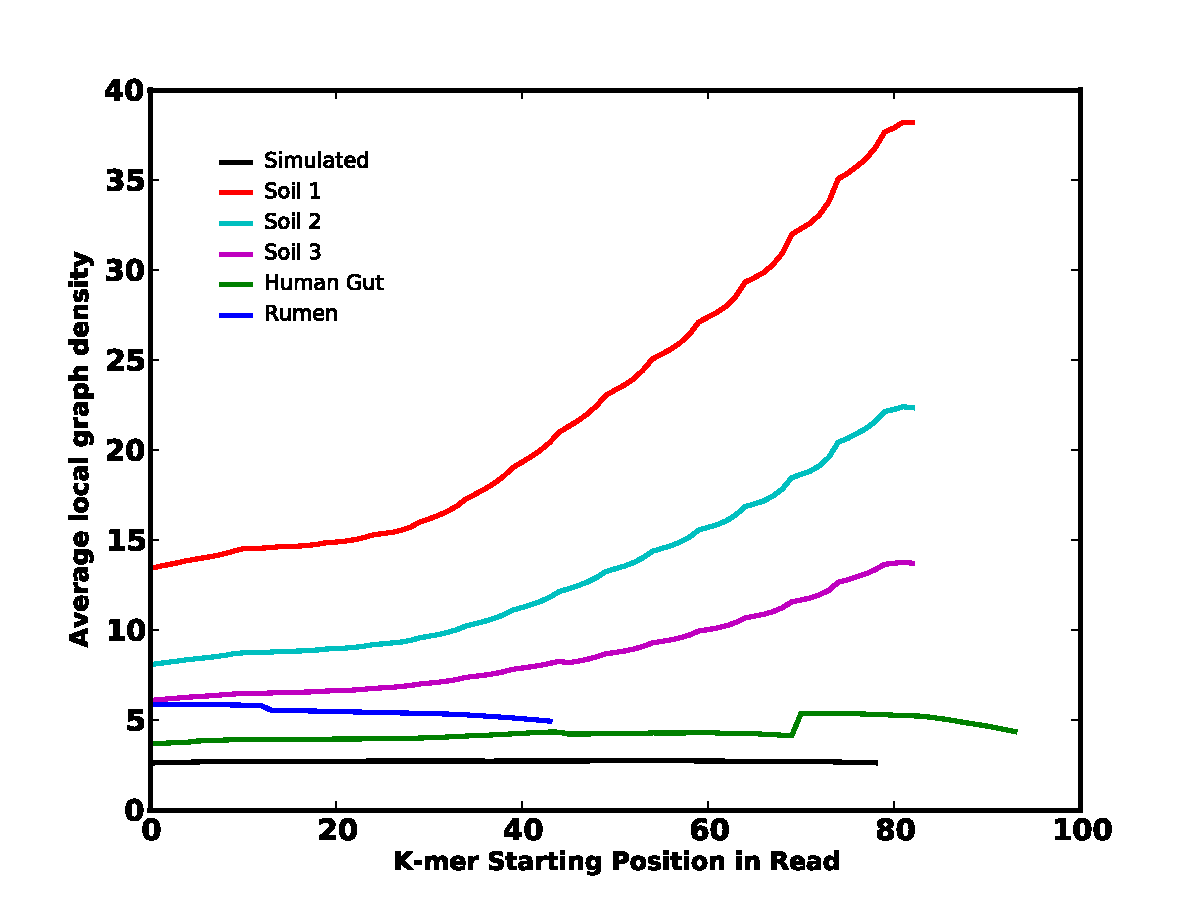
\includegraphics[width=5in]{./Figures/figure1-density.pdf}}
\caption{The extent to which average local graph density varies by read position is shown for the lump of various datasets.}
\end{figure}

\begin{figure}
\center{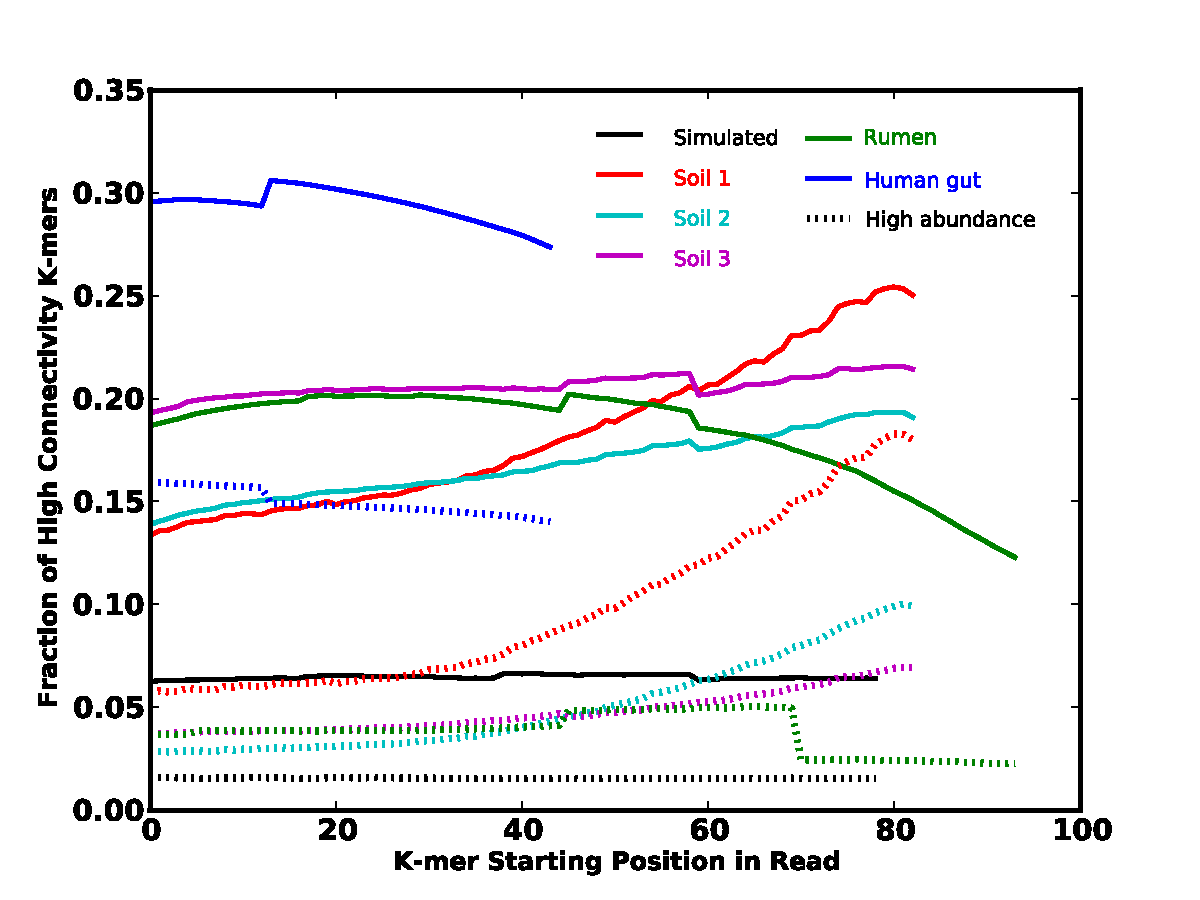
\includegraphics[width=5in]{./Figures/figure2-hckmers.pdf}}
\caption{The extent to which highly connecting k-mers (solid lines) and the subset of highly abundant (greater than 50) k-mers (dashed lines) are present at specific positions within sequencing reads for various metagenomes.}
\end{figure}

\begin{figure}
\center{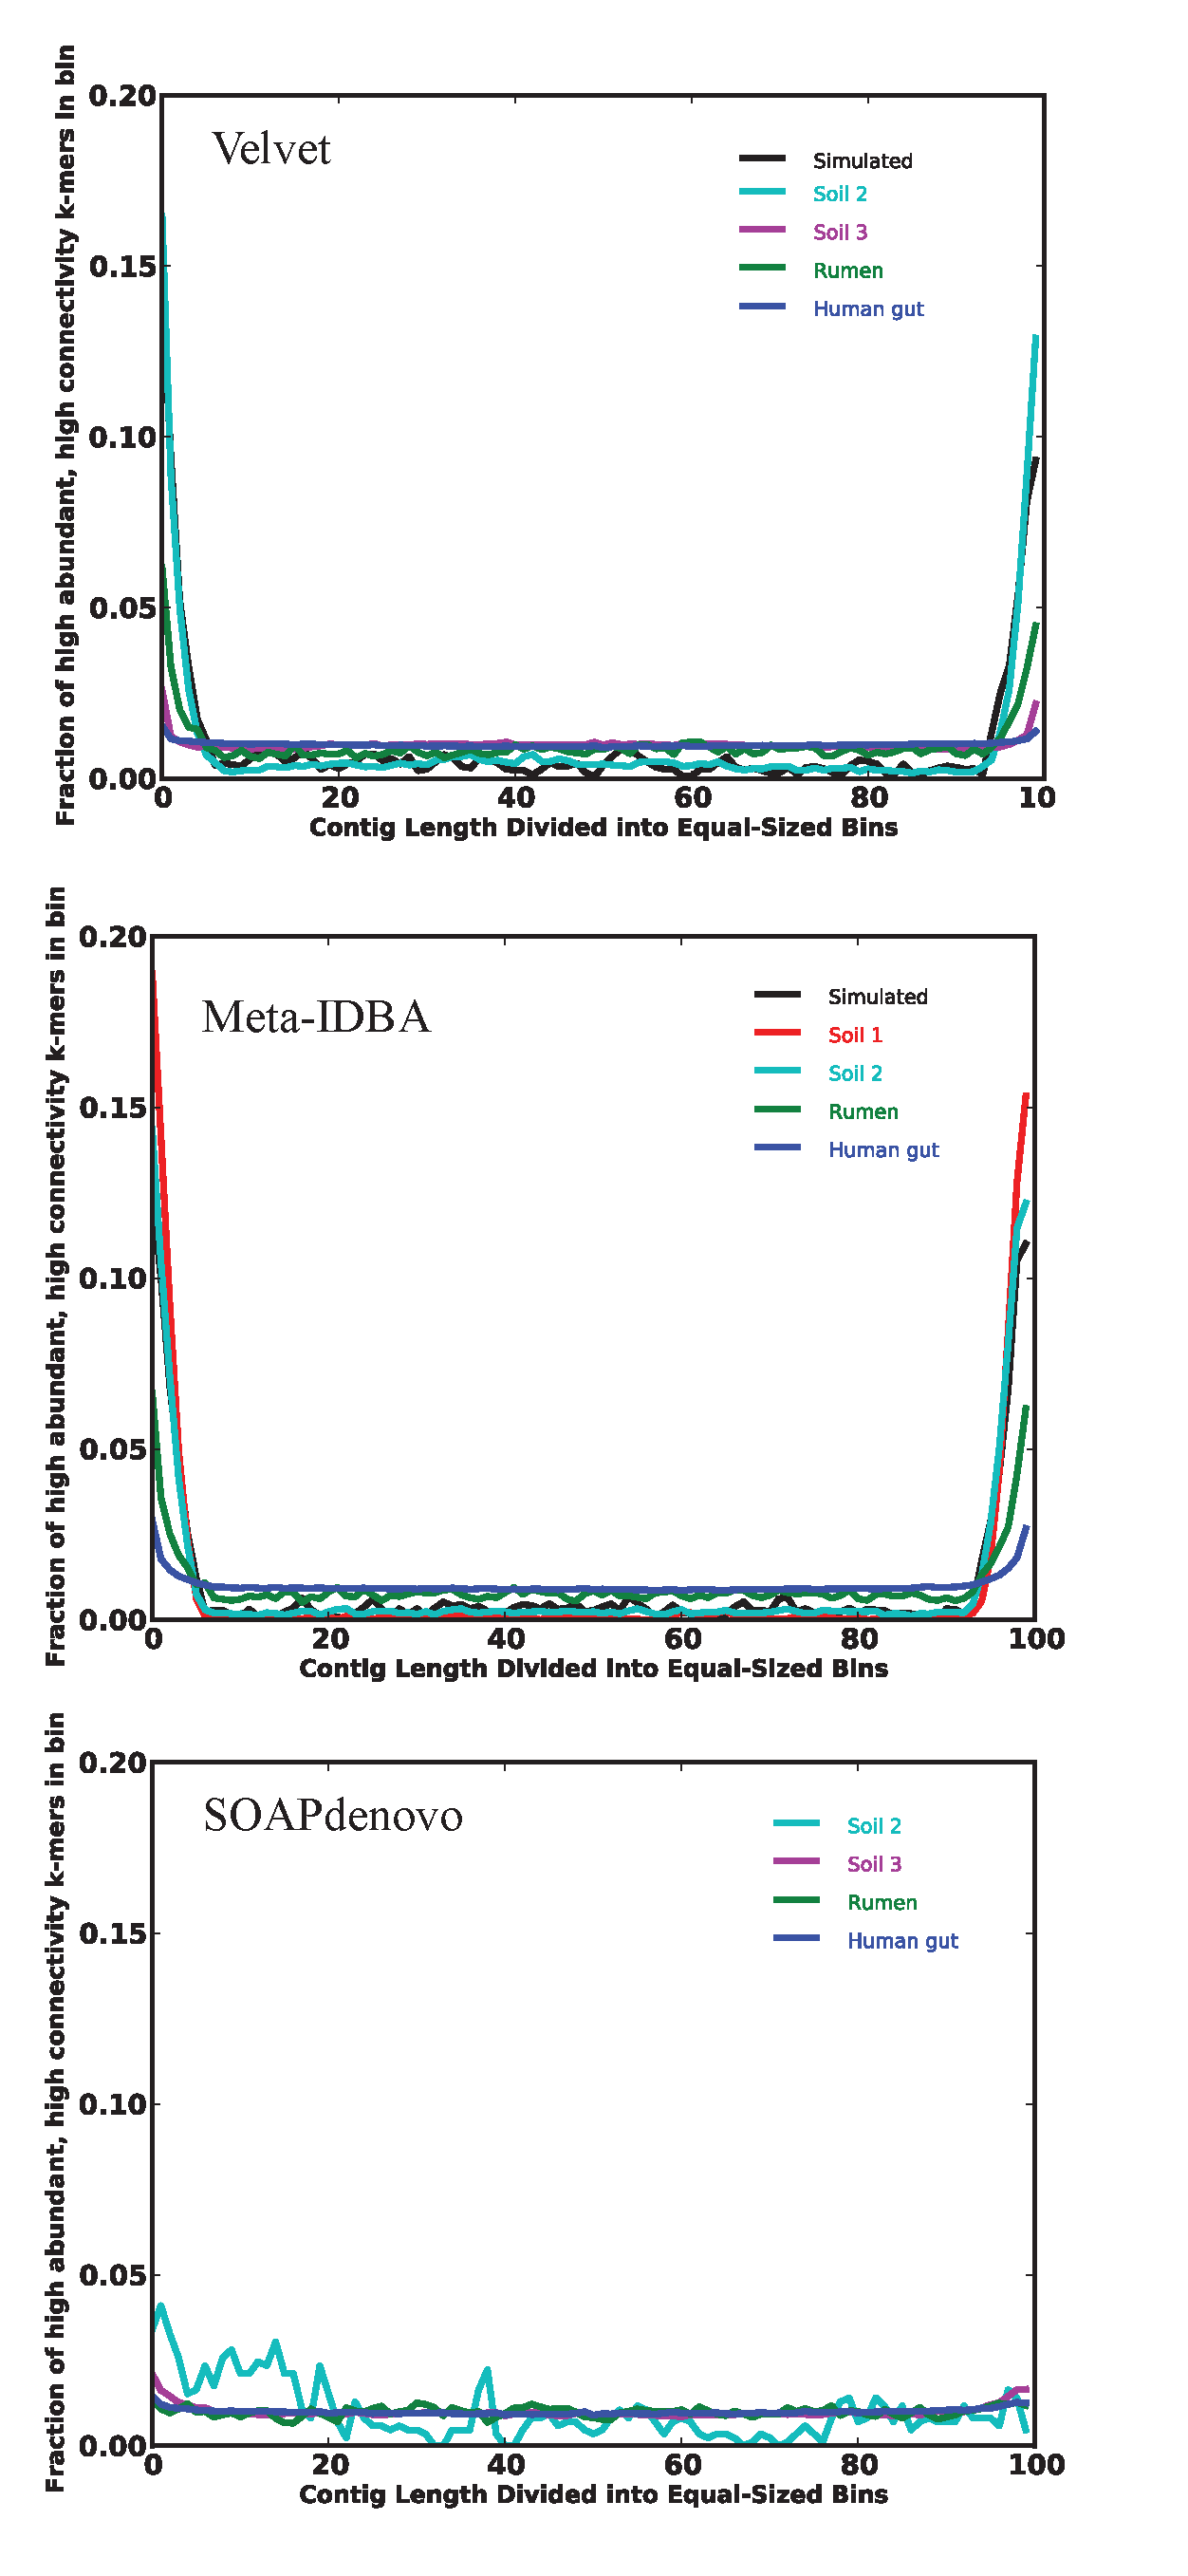
\includegraphics[width=\textwidth,height=\textheight,keepaspectratio]{./Figures/figure3-contigs.pdf}}
\caption{When incorporated into an assembly, abundant (greater than 50 times), highly connecting sequences (k-mers) were disproportionately present at the ends of contigs.  The total fraction of highly connecting k-mers which are incorporated into each contig binned region.}
\end{figure}

\begin{figure}
\center{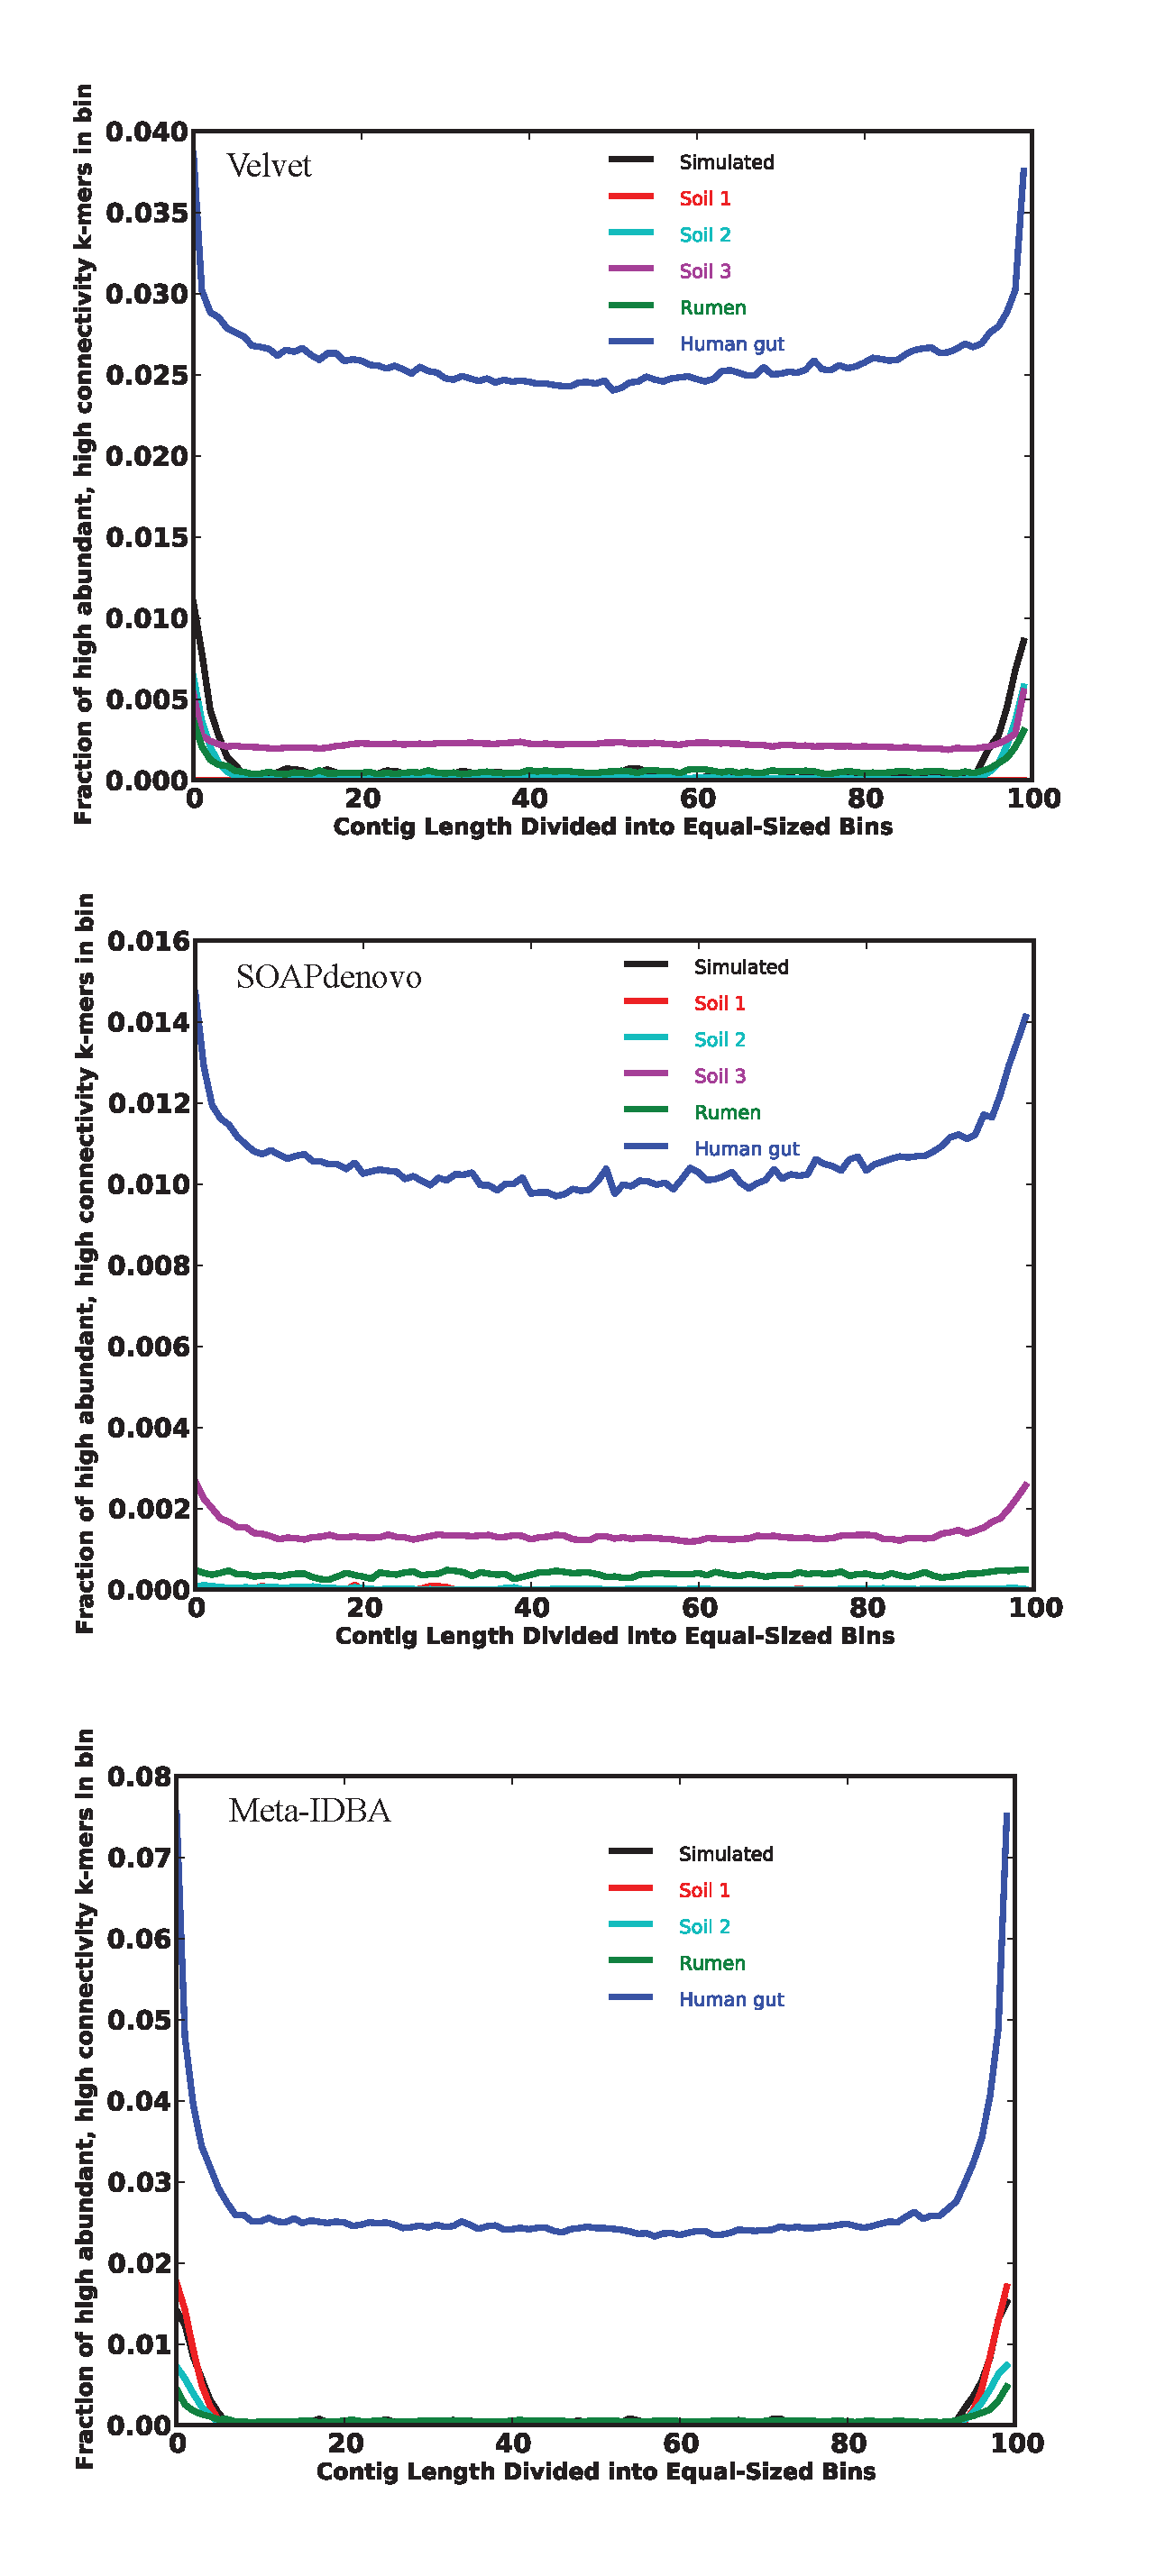
\includegraphics[width=\textwidth,height=\textheight,keepaspectratio]{./Figures/figure4-contigs.pdf}}
\caption{When incorporated into an assembly, abundant (greater than 50 times), highly connecting sequences (k-mers) were disproportionately present at the ends of contigs.  We show the total fraction of all k-mers which are identified as high abundance/high connectivity sequences and incorporated into each contig.}
\end{figure}

\begin{figure}
\center{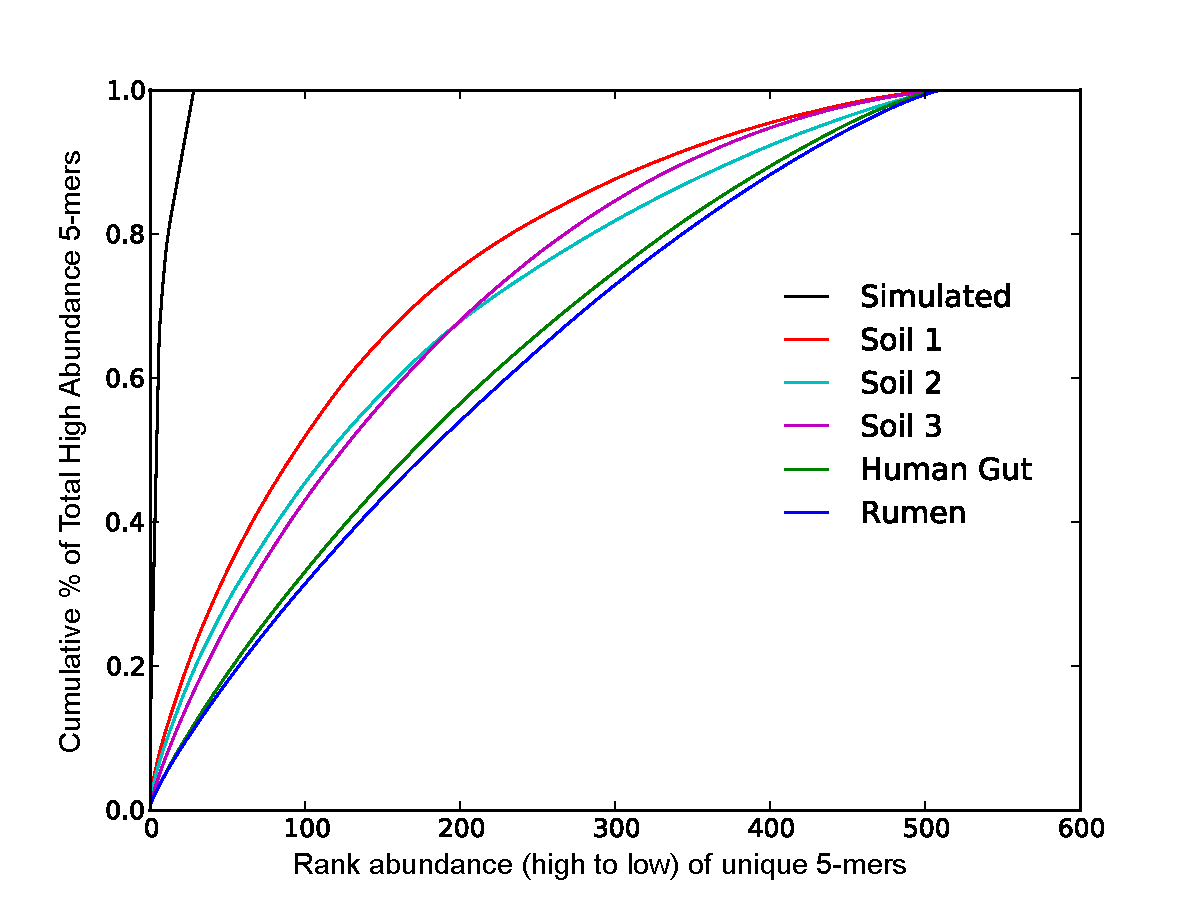
\includegraphics[width=\textwidth,height=\textheight,keepaspectratio]{./Figures/figure5-5mers.pdf}}
\caption{Rank abundance plot of 5-mers present in abundant, highly connected sequences in various datasets.}
\end{figure}
\end{document}









